\documentclass[12pt,a4paper]{article}
\usepackage{rmpackages}																% usual packages
\usepackage{rmtemplate}																% graphic charter
\usepackage{rmexocptce}																% for DS with cptce eval

%\cfoot{} 													% if no page number is needed
%\renewcommand\arraystretch{1.5}		% stretch table line height

\begin{document}

\begin{header}
Devoir à la maison 2
\end{header}

Pour revoir les points essentiels du chapitre 5 en vidéo, un extrait de l'émission C'est pas sorcier : \href{https://youtu.be/Q58ns2rLXx8}{https://youtu.be/Q58ns2rLXx8}.

\section*{Vacarme animalier}

\begin{doc}
\textbf{La cigale}
\vspace{-\baselineskip}
\begin{multicols}{2}
\begin{center}
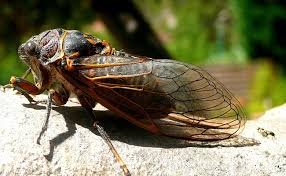
\includegraphics[width=0.45\textwidth]{images/cigale.jpg}
\end{center}

Les cigales sont les insectes les plus bruyants du monde.
Elles émettent leur chant à l'aide d'organes situés de chaque côté du corps et appelés des timbales.
Des contractions musculaires répétitives font vibrer ces timbales.
Leur abdomen creux leur permet d'émettre des sons dont le niveau d'intensité sonore atteint \unit{120}{dB}.
\end{multicols}
\end{doc}

\begin{multicols}{2}
\begin{doc}
\textbf{Le grand dauphin}
\begin{center}
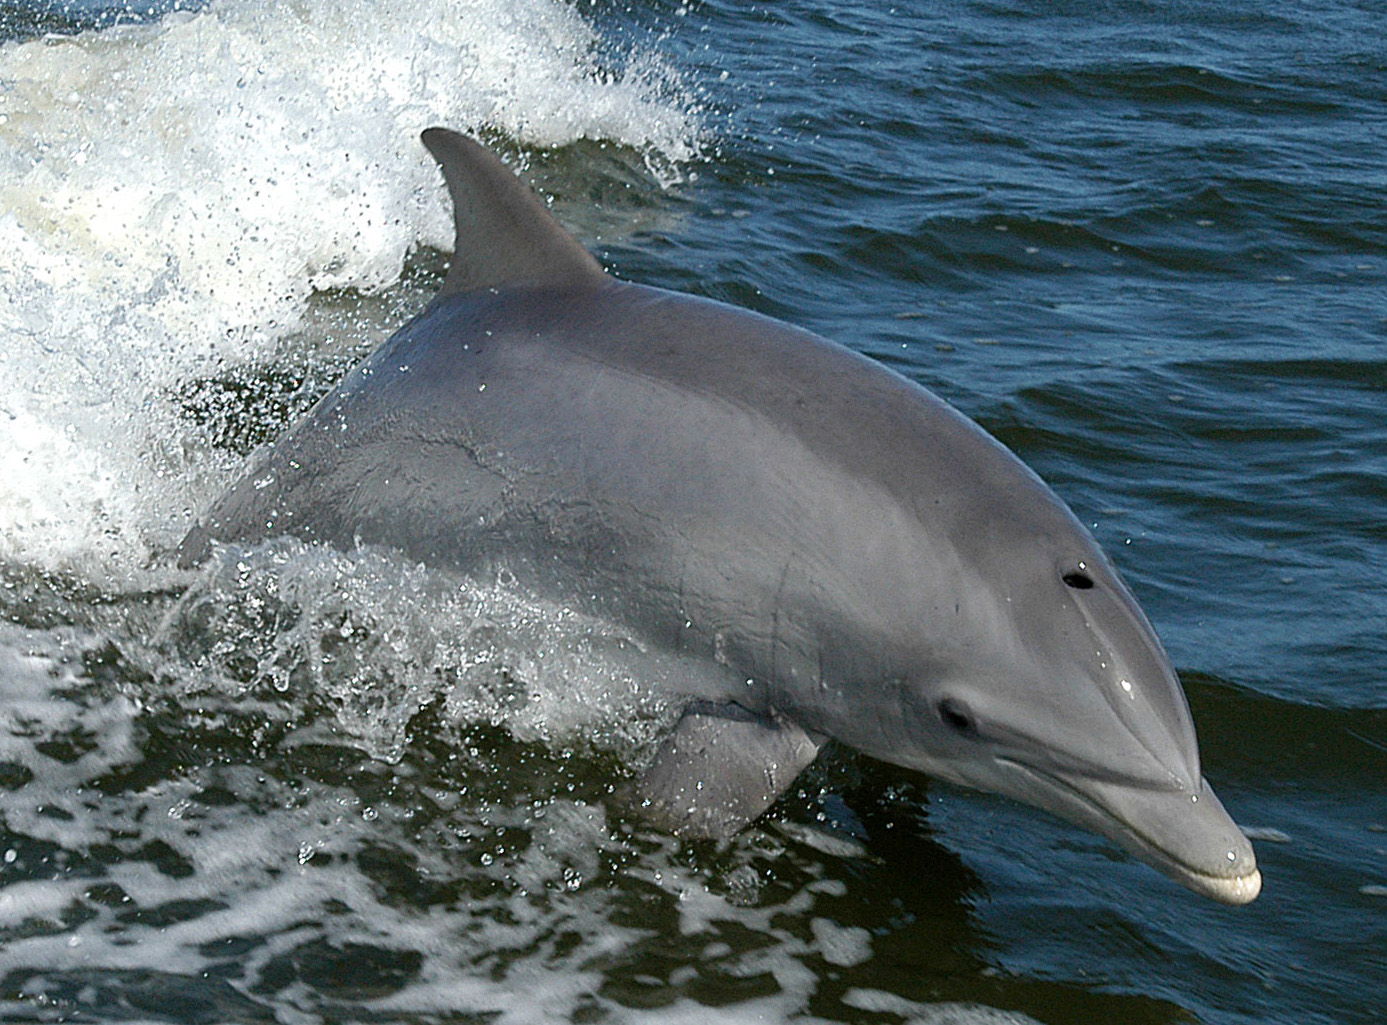
\includegraphics[width=\textwidth]{images/dauphin.jpg}
\end{center}
Le dauphin est un excellent chasseur : il utilise l'écholocalisation.
Pour repérer ses proies, il émet des clics sonores de fréquence voisine de \unit{220}{kHz} et dont le niveau d'intensité sonore peut dépasser \unit{220}{dB}.
\end{doc}

\begin{doc}
\textbf{L'éléphant}
\begin{center}
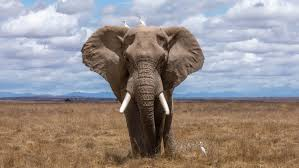
\includegraphics[width=\textwidth]{images/elephant.jpg}
\end{center}
Pour communiquer sur de longues distances, les éléphants utilisent des infrasons dont le niveau d'intensité sonore est proche de \unit{100}{dB}.
\end{doc}
\end{multicols}

\begin{enumerate}
\item La manière dont la cigale émet son chant se rapproche du fonctionnement du diapason (composé d'une fourche et d'une caisse de résonance).
Chez la cigale, quel organe joue le rôle de la fourche du diapason ?
Et de celui de la caisse de résonance ?

\item D'après les documents, indiquer en le justifiant qui de la cigale, du dauphin ou de l'éléphant émet le son le plus fort.

\item Les deux signaux du Doc.~\ref{doc:records} sont des enregistrements du son émis par un dauphin et un éléphant, mais la personne en charge des mesures a maladroitement nommé les enregistrements \og Animal 1 \fg{} et \og Animal 2 \fg{}.
Attribuer chaque enregistrement au bon animal.

\emph{Pour répondre à cette question, mettre en œuvre les étapes de la démarche scientifique : reformulation, hypothèse, protocole et conclusion.}

\item Le timbre de ces deux sons est-il le même ?
Et la hauteur ?
\end{enumerate}

\begin{doc}
\label{doc:records}
\textbf{Enregistrements sonores}

\noindent
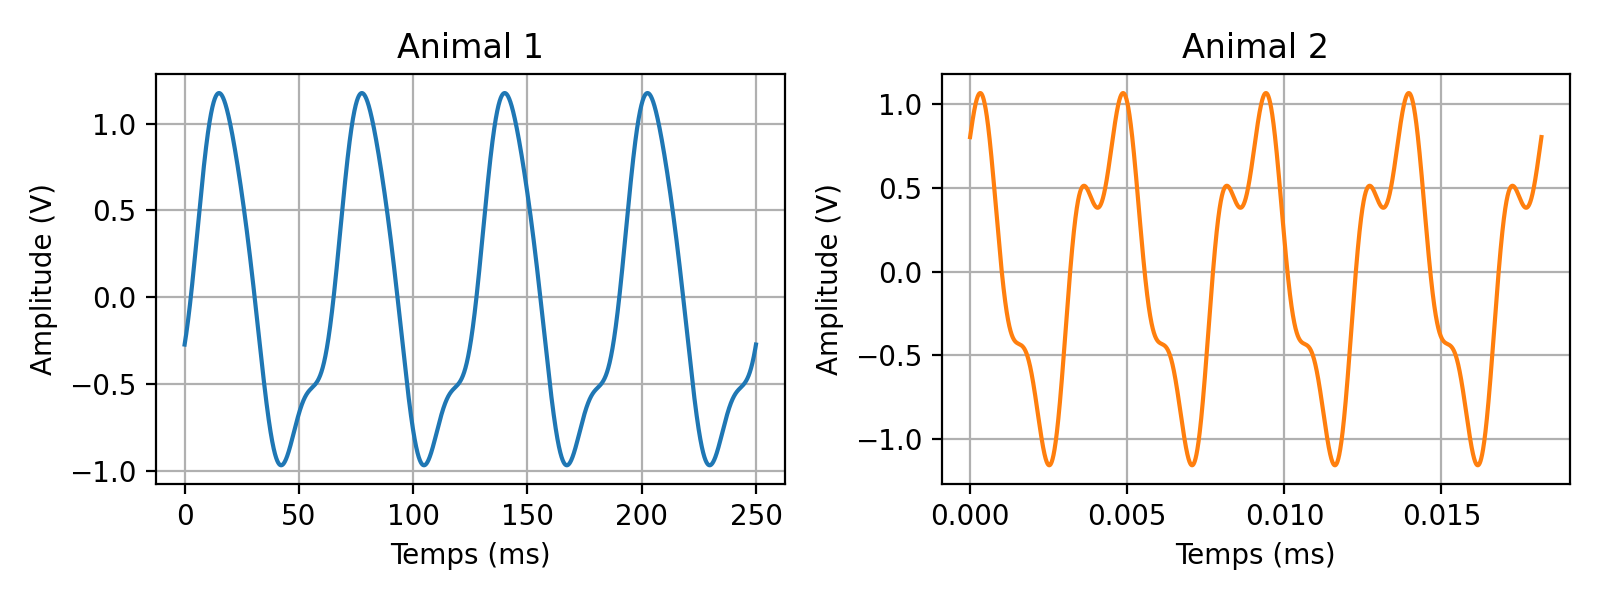
\includegraphics[width=\textwidth]{images/animals.png}
\end{doc}

\section*{L'effet Donald Duck}

Regarder le cours extrait vidéo de l'émission Mythbusters \href{https://youtu.be/JjJOS0BpgnM}{https://youtu.be/JjJOS0BpgnM}.
Les sous-titres français sont disponibles.

\begin{enumerate}[resume]
\item Quel gaz permet d'obtenir une voix plus aigüe ?
Une voix plus grave ?

\item D'après la vidéo, dans quel gaz le son se propage-t-il le plus rapidement ?

\item Dans l'hélium, le son parcours \unit{350}{m} en \unit{0{,}34}{s}.
Calculer la vitesse du son dans l'hélium.
\label{quest:son_he}

\item Dans l'hexafluorure de soufre le son parcours \unit{1{,}0}{m} en \unit{7{,}5}{ms}.
Calculer la vitesse du son dans l'hexafluorure de soufre.
\label{quest:son_sf6}

\item Comparer les valeurs obtenues à la vitesse du son dans l'air.

\item Les résultats des questions~\ref{quest:son_he} et \ref{quest:son_sf6} sont-il en accord avec les affirmations de la vidéo ?

\end{enumerate}

\paragraph{Bonus :}
\begin{itemize}
\item[•] les trente premières secondes d'une scène du Grand bleu : \href{https://youtu.be/WIrMEgJDZV0}{https://youtu.be/WIrMEgJDZV0} ;
\item[•] Sofia Vergara (en anglais) : \href{https://youtu.be/hDuIovlDTGU?t=52}{https://youtu.be/hDuIovlDTGU?t=52} ;
\item[•] Jennifer Lawrence, Will Ferrell, etc. (en anglais) : \href{https://youtu.be/vBIYUeiKAXU?t=5}{https://youtu.be/vBIYUeiKAXU?t=5}.
\end{itemize}


\end{document}